\chapter{Background}
\label{chp:background}

This chapter will cover the cryptographic background of the necessary components in order to understand CryptDB, along with some of the basic cryptographic principals.

...More. Symmetric/Asymmetric/ has no references. Is this trivial enough to go without?

\section{Symmetric Encryption}

Symmetric key encryption is, perhaps, the most intuitive type of encryption, where the sender encrypts the data with a secret key that the sender and receiver has agreed upon in advance. When receiving data, the receiver uses the pre-shared secret key in order to decrypt the data. In a more formal matter, symmetric key encryption is usually used either with a block cipher(which encrypts messages in chunks of data) or a stream cipher (which encrypts data bit-by-bit). The scheme usually consist of three algorithms, $KeyGen$, $Enc$ and $Dec$.

$KeyGen$ is the algorithm that generates the secret key $k_s$ used for encryption and decryption, $Enc_k$ encrypts the data with the secret key, and $Dec_k$ decrypts it using the same secret key. One of the major drawbacks with symmetric key cryptography is that the secret key $k_s$ needs to be shared between the parties that are communicating. If an adversary obtains the secret key, say that one of the parties stored it on a piece of paper that was misplaced and lost, the whole communication channel would be compromised as the adversary could easily decrypt the data.

In database systems, symmetric encryption is often used to store data by encrypting it under some secret key $k_s$ that is kept in the database. Given that the information in the database is stored using the same key, this approach provides little security against unauthorized users that gain access to the secret key. On the plus side, the process of encrypting data using a symmetric encryption scheme is usually fast compared to other approaches that uses multiple keys.


\section{Asymmetric Encryption}

In contrast to symmetric key encryption, asymmetric key encryption does not depend on a pre-shared secret key. Asymmetric key encryption, or Public-Key Encryption, is based upon the fact that some mathematical problems are considered \emph{hard}, such as the integer factorization, discrete logarithms and elliptic curves. By computing a key-pair consisting of a public key and a private key, two users are able to exchange keys over a public channel without worrying about their secret keys being compromised.

The public key is used for encrypting data sent to the user, and the private key is used to decrypt received data that is encrypted with said public key. Two of the most recognized public-key cryptosystems are \gls{rsa}, which relies of the integer factorization problem, and ElGamal, which relies on the discrete logarithms problem. In addition to secure communication between multiple parties, public key cryptography is also applied to create digital signatures, which provides authentication and data integrity.

For applications using databases that are storing information for different users, asymmetric encryption would be a natural encryption scheme. Information sent from one user to another could be encrypted under the receivers public key and vice-versa, and decrypted by applying their secret keys.

% Why are we talking about asymmetric encryption?

\section{Homomorphic Encryption}

We love to describe encryption as safes where we store our data, then secures it with one or more locks, and hide the secret key. Without the secret key, the data is securely stored inside the safe. Whenever we need our data, we take the hidden key out from its hideout and opens all the locks of the safe, where the data is as intact as we left it. The, perhaps, holiest of all the holy grails in cryptography is called \emph{homomorphic encryption}. This is a special case of encryption where operations on the encrypted data are possible without decrypting it first, or in the perspective of our locked safe: Modify the data on the inside of the safe without ever unlocking it. Figure \ref{fig:he_ill} illustrates the main concept of homomorphic encryption used in a cloud service scenario.

\begin{figure}[h]
	\centering
	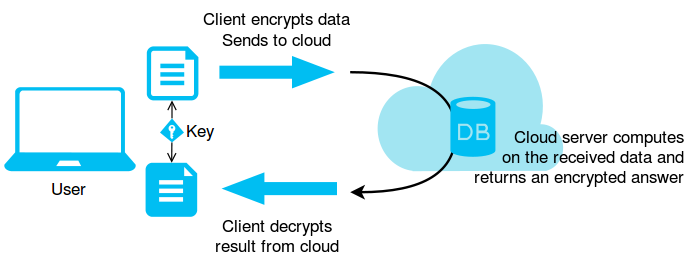
\includegraphics[scale=0.5]{he.png}
	\caption{Illustration of a homomorphic system where data is encrypted at the client, sent to the server which performs computation on the encrypted data and returns an encrypted result which is decrypted by the client.}
	\label{fig:he_ill}
\end{figure}

Regular \gls{pke} schemes consists of three algorithms, namely a key generation algorithm (\texttt{KeyGen}), an encryption algorithm (\texttt{Enc}) and a decryption algorithm (\texttt{Dec}). \gls{he} schemes adds another algorithm to the toolbox, an evaluation algorithm (\texttt{Eval}).  Assume a well formed public key $pk$, a boolean circuit $C$ and a set of ciphertexts $c_1, ..., c_l$ which are encryptions of $m_1, ..., m_l$ respectively. Then \texttt{Eval} outputs a ciphertext $c$ which encrypted under $pk$ such that $Dec_{sk}(c) = C(m_1, ..., m_l)$ for some secret key $sk$ \cite{damgaard2012secure}.


For \gls{phe} schemes, $Eval$ will be associated to a set of permitted functions $f$ (or circuits). These are functions that the algorithm can handle, and which guarantee a meaningful result when executed. These functions can be expressed as boolean circuits consisting of logical gates such as AND, OR and NOT. Gentry \cite{Gentry_computing_arb_func_enc_data} presented a homomorphic encryption scheme consisting of three functions; addition ($Add_{\epsilon}$), subtraction ($Sub_{\epsilon}$) and multiplication ($Mult_{\epsilon}$). When performing homomorphic operations using functions from $f$, an N-bit noise is generated and added to the encrypted ciphertext, making the relation between the encrypted result and its corresponding plaintext weaker. By performing multiple operations on the ciphertexts, the noise grows larger. Problems arise when the noisy part gets too large, as the decryption algorithm might not be able to decrypt in a reliable way in order to obtain the correct result.

\section{Fully Homomorphic Encryption}

\Gls{fhe}, which has no restrictions to what types of operations that can be performed on the encrypted data, was first suggested in 1978 by Rivest, Adleman, and Dertouzos \cite{rivest1978data}. At this point in time, researchers did not have any secure scheme for using these ideas. More importantly, there were not many use cases driving the need of such schemes. It has therefore been a slightly displaced and forgotten grail until 2009,
when Gentry presented the first \gls{fhe} scheme based on lattices \cite{Gentry_first_lattices}, and a year later another scheme using a \emph{bootstrappable} approach \citep{Gentry_computing_arb_func_enc_data}. Nearly all modern \gls{fhe} schemes are based on this bootstrappable concept using Gentry's blueprints. 

As mentioned in the section above, a homomorphic operation creates noise when executed. Multiple operations adds more noise which may change the decrypted result beyond the recognizable. But what if we had a scheme that was able to reduce the noise generated by such operations? Boostrapping involves encrypting the secret key $sk$ under its corresponding public key $pk$ and added to a modified encryption algorithm, $Recrypt(pk_{i+1}, D_{\epsilon}, \overline{sk_i}, c_i)$. This basically enables the algorithm to decrypt the ciphertext $c_i$ taken as input internally while being encrypted under the new public key $pk_{i+1}$. $Recrypt$ returns a \emph{freshly} created ciphertext $c_{i+1}$ which is less noise than the original $c_1$ ciphertext to continue to perform homomorphic operations on.

Equation \ref{enc_m} encrypts the message $m$ under the public key $pk_1$ as most asymmetric encryption schemes does, in order to obtain the ciphertext $c_1$. So far, nothing we have not seen before. Now, the secret key $sk_1$ from the public-key-pair $(pk_1,sk_1)$ is encrypted using a new, fresh public-key pair $(pk_2, sk_2)$ as seen in Equation \ref{enc_sk}. By doing so, the algorithm enables $Eval$ to later on decrypt $c_1$ using $sk_1$ while under the encryption of $pk_2$.

\begin{equation}
\label{enc_m}
c_1 = Enc(pk_1, m)
\end{equation}
\begin{equation}
\label{enc_sk}
\overline{sk_1} = Enc(pk_2, sk_1)
\end{equation}


Bootstrapping works recursively, so for the algorithm to be able to decrypt the $c_1$ in the next iteration, it needs to be encrypted under the new public key $pk_2$ as seen in Equation \ref{enc_c_1}. In Equation \ref{eval_c1_pk2}, a new and fresh ciphertext is produced by the $Eval$ algorithm, which uses $pk_2$ to encrypt the noisy ciphertext $c_1$, and D to decrypt it $c_1$ using its corresponding $sk_1$ inside $Eval$. By doing this, the noise of the ciphertext is reduced, while still being encrypted - Now under the public key $pk_2$. Figure \ref{recrypt_function} shows the process of the $Recrypt$ algorithm.

%% Dette er piss. 


\begin{equation}
\label{enc_c_1}
\overline{c_1} = Enc(pk_2, c_1)
\end{equation}
\begin{equation}
\label{eval_c1_pk2}
c_1' = Eval(pk_2, D_{\epsilon}, \overline{sk_1}, \overline{c_1})
\end{equation}


\begin{figure}[h]
	\centering
	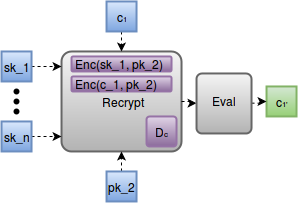
\includegraphics[scale=0.8]{bootstrapp.png}
	\caption{Illustration of the Recrypt algorithm, which refreshes the ciphertext $c_1$ encrypted under the new public key $p_2$.}
	\label{recrypt_function}
\end{figure}



When allowing the encryption function to handle its own decryption function at the same time, Gentry showed that the noise added by the homomorphic operations was less than the noise removed by the additional decryption \cite{Gentry_computing_arb_func_enc_data}, and the breakthrough was made in hunt for a fully homomorphic encryption scheme. While Gentry's system is great in theory, it has been shown that creating \gls{fhe} schemes is hard in practice. However, some other cryptographic schemes holds different types of homomorphic properties which when combined can provide different homomorphic operations. Addition is, for example, a homomorphic property of the Pailler cryptosystem \citep{Paillier}. Pailler is originally a trapdoor mechanism based on the Composite Residuosity Class Problem which conveniently has the cryptographic property such that \[ENC_k(x) * ENC_k(y) = ENC_k(x + y)\]

Another practical cryptosystem providing a similar property, is the ElGamal cryptosystem \cite{elgamal}. Along with being an asymmetric cryptosystem , it has the cryptographic property shown below, which enables it to perform homomorphic multiplications.  \[ENC_k(x) * ENC_k(y) = ENC(x * y)\]


\section{Database Security}
\label{chp:database_Security}

Databases are central building blocks in most computer systems, allowing data to be stored, shared, and read by users. As the amount of data stored does not decrease over time, database systems experience an exponential growth. There are companies that stores banking information, health records, and other sensitive information, which makes them a target for criminals and hackers. In order to cope with such attacks, systems that are relying on some sort of database structure, are in need of defence mechanisms. 


Most database systems are stored behind different network security measures such as firewalls and intrusion detection systems. A database firewall will, for example, monitor all traffic to and from a database system in order to detect situations that deflects from the predetermined database policy. Such measures does however only provide security for the outside of the system, but a system is in need of security on the inside as well. Most database systems provide different security measures for handling situations that can occur on the inside.

Access control is used for granting different privileges for a user or user groups to a certain object in the database, such as a table, view or procedure. Authentication is used to ensure that only trusted entities are able to reach the database, and to grant the correct privileges based on the identity of the user. For applications where certain user groups are handling sensitive information, a person in charge of the system may have the need to monitor who accessed a given table at a certain time in case of information leaks and similar circumstances. Auditing is a database security technique which does not directly prevent security protocols from being broken, but allows the system administrator to backtrack and discover breaches in the security.

Another vital part of keeping a database secure, is of course the use of database encryption. Both symmetric and asymmetric encryption is possible to perform on database systems, and there exists different ways of layering the encryption based on the application.


Hmm. Not sure about how good this section is. What to add, remove, etc?